%
\begin{isabellebody}%
\def\isabellecontext{Examples{\isadigit{3}}}%
%
\isadelimtheory
%
\endisadelimtheory
%
\isatagtheory
\isacommand{theory}\isamarkupfalse%
\ Examples{\isadigit{3}}\isanewline
\isakeyword{imports}\ Examples\ {\isachardoublequoteopen}{\isachartilde}{\isachartilde}{\isacharslash}src{\isacharslash}HOL{\isacharslash}Number{\isacharunderscore}Theory{\isacharslash}UniqueFactorization{\isachardoublequoteclose}\isanewline
\isakeyword{begin}%
\endisatagtheory
{\isafoldtheory}%
%
\isadelimtheory
\isanewline
%
\endisadelimtheory
%
\isadeliminvisible
%
\endisadeliminvisible
%
\isataginvisible
\isacommand{hide}\isamarkupfalse%
\ const\ Lattices{\isachardot}lattice%
\endisataginvisible
{\isafoldinvisible}%
%
\isadeliminvisible
%
\endisadeliminvisible
%
\begin{isamarkuptext}%
\vspace{-5ex}%
\end{isamarkuptext}%
\isamarkuptrue%
%
\isamarkupsubsection{Third Version: Local Interpretation
  \label{sec:local-interpretation}%
}
\isamarkuptrue%
%
\begin{isamarkuptext}%
In the above example, the fact that \isa{op\ {\isasymle}} is a partial
  order for the natural numbers was used in the second goal to
  discharge the premise in the definition of \isa{op\ {\isasymsqsubset}}.  In
  general, proofs of the equations not only may involve definitions
  fromthe interpreted locale but arbitrarily complex arguments in the
  context of the locale.  Therefore is would be convenient to have the
  interpreted locale conclusions temporary available in the proof.
  This can be achieved by a locale interpretation in the proof body.
  The command for local interpretations is \isakeyword{interpret}.  We
  repeat the example from the previous section to illustrate this.%
\end{isamarkuptext}%
\isamarkuptrue%
%
\isadelimvisible
\ \ %
\endisadelimvisible
%
\isatagvisible
\isacommand{interpretation}\isamarkupfalse%
\ nat{\isacharcolon}\ partial{\isacharunderscore}order\ {\isachardoublequoteopen}op\ {\isasymle}\ {\isacharcolon}{\isacharcolon}\ nat\ {\isasymRightarrow}\ nat\ {\isasymRightarrow}\ bool{\isachardoublequoteclose}\isanewline
\ \ \ \ \isakeyword{where}\ {\isachardoublequoteopen}partial{\isacharunderscore}order{\isachardot}less\ op\ {\isasymle}\ {\isacharparenleft}x{\isacharcolon}{\isacharcolon}nat{\isacharparenright}\ y\ {\isacharequal}\ {\isacharparenleft}x\ {\isacharless}\ y{\isacharparenright}{\isachardoublequoteclose}\isanewline
\ \ \isacommand{proof}\isamarkupfalse%
\ {\isacharminus}\isanewline
\ \ \ \ \isacommand{show}\isamarkupfalse%
\ {\isachardoublequoteopen}partial{\isacharunderscore}order\ {\isacharparenleft}op\ {\isasymle}\ {\isacharcolon}{\isacharcolon}\ nat\ {\isasymRightarrow}\ nat\ {\isasymRightarrow}\ bool{\isacharparenright}{\isachardoublequoteclose}\isanewline
\ \ \ \ \ \ \isacommand{by}\isamarkupfalse%
\ unfold{\isacharunderscore}locales\ auto\isanewline
\ \ \ \ \isacommand{then}\isamarkupfalse%
\ \isacommand{interpret}\isamarkupfalse%
\ nat{\isacharcolon}\ partial{\isacharunderscore}order\ {\isachardoublequoteopen}op\ {\isasymle}\ {\isacharcolon}{\isacharcolon}\ {\isacharbrackleft}nat{\isacharcomma}\ nat{\isacharbrackright}\ {\isasymRightarrow}\ bool{\isachardoublequoteclose}\ \isacommand{{\isachardot}}\isamarkupfalse%
\isanewline
\ \ \ \ \isacommand{show}\isamarkupfalse%
\ {\isachardoublequoteopen}partial{\isacharunderscore}order{\isachardot}less\ op\ {\isasymle}\ {\isacharparenleft}x{\isacharcolon}{\isacharcolon}nat{\isacharparenright}\ y\ {\isacharequal}\ {\isacharparenleft}x\ {\isacharless}\ y{\isacharparenright}{\isachardoublequoteclose}\isanewline
\ \ \ \ \ \ \isacommand{unfolding}\isamarkupfalse%
\ nat{\isachardot}less{\isacharunderscore}def\ \isacommand{by}\isamarkupfalse%
\ auto\isanewline
\ \ \isacommand{qed}\isamarkupfalse%
%
\endisatagvisible
{\isafoldvisible}%
%
\isadelimvisible
%
\endisadelimvisible
%
\begin{isamarkuptext}%
The inner interpretation is immediate from the preceding fact
  and proved by assumption (Isar short hand ``.'').  It enriches the
  local proof context by the theorems
  also obtained in the interpretation from Section~\ref{sec:po-first},
  and \isa{nat{\isachardot}less{\isacharunderscore}def} may directly be used to unfold the
  definition.  Theorems from the local interpretation disappear after
  leaving the proof context --- that is, after the closing a
  \isakeyword{next} or \isakeyword{qed} statement.%
\end{isamarkuptext}%
\isamarkuptrue%
%
\isamarkupsubsection{Further Interpretations%
}
\isamarkuptrue%
%
\begin{isamarkuptext}%
Further interpretations are necessary for
  the other locales.  In \isa{lattice} the operations \isa{{\isasymsqinter}} and
  \isa{{\isasymsqunion}} are substituted by \isa{min} and
  \isa{max}.  The entire proof for the
  interpretation is reproduced to give an example of a more
  elaborate interpretation proof.%
\end{isamarkuptext}%
\isamarkuptrue%
%
\isadelimvisible
\ \ %
\endisadelimvisible
%
\isatagvisible
\isacommand{interpretation}\isamarkupfalse%
\ nat{\isacharcolon}\ lattice\ {\isachardoublequoteopen}op\ {\isasymle}\ {\isacharcolon}{\isacharcolon}\ nat\ {\isasymRightarrow}\ nat\ {\isasymRightarrow}\ bool{\isachardoublequoteclose}\isanewline
\ \ \ \ \isakeyword{where}\ {\isachardoublequoteopen}lattice{\isachardot}meet\ op\ {\isasymle}\ {\isacharparenleft}x{\isacharcolon}{\isacharcolon}nat{\isacharparenright}\ y\ {\isacharequal}\ min\ x\ y{\isachardoublequoteclose}\isanewline
\ \ \ \ \ \ \isakeyword{and}\ {\isachardoublequoteopen}lattice{\isachardot}join\ op\ {\isasymle}\ {\isacharparenleft}x{\isacharcolon}{\isacharcolon}nat{\isacharparenright}\ y\ {\isacharequal}\ max\ x\ y{\isachardoublequoteclose}\isanewline
\ \ \isacommand{proof}\isamarkupfalse%
\ {\isacharminus}\isanewline
\ \ \ \ \isacommand{show}\isamarkupfalse%
\ {\isachardoublequoteopen}lattice\ {\isacharparenleft}op\ {\isasymle}\ {\isacharcolon}{\isacharcolon}\ nat\ {\isasymRightarrow}\ nat\ {\isasymRightarrow}\ bool{\isacharparenright}{\isachardoublequoteclose}%
\begin{isamarkuptxt}%
\normalsize We have already shown that this is a partial
	order,%
\end{isamarkuptxt}%
\isamarkuptrue%
\ \ \ \ \ \ \isacommand{apply}\isamarkupfalse%
\ unfold{\isacharunderscore}locales%
\begin{isamarkuptxt}%
\normalsize hence only the lattice axioms remain to be
	shown: \begin{isabelle}%
\ {\isadigit{1}}{\isachardot}\ {\isasymAnd}x\ y{\isachardot}\ {\isasymexists}inf{\isachardot}\ partial{\isacharunderscore}order{\isachardot}is{\isacharunderscore}inf\ op\ {\isasymle}\ x\ y\ inf\isanewline
\ {\isadigit{2}}{\isachardot}\ {\isasymAnd}x\ y{\isachardot}\ {\isasymexists}sup{\isachardot}\ partial{\isacharunderscore}order{\isachardot}is{\isacharunderscore}sup\ op\ {\isasymle}\ x\ y\ sup%
\end{isabelle}  After unfolding \isa{is{\isacharunderscore}inf} and
	\isa{is{\isacharunderscore}sup},%
\end{isamarkuptxt}%
\isamarkuptrue%
\ \ \ \ \ \ \isacommand{apply}\isamarkupfalse%
\ {\isacharparenleft}unfold\ nat{\isachardot}is{\isacharunderscore}inf{\isacharunderscore}def\ nat{\isachardot}is{\isacharunderscore}sup{\isacharunderscore}def{\isacharparenright}%
\begin{isamarkuptxt}%
\normalsize the goals become \begin{isabelle}%
\ {\isadigit{1}}{\isachardot}\ {\isasymAnd}x\ y{\isachardot}\ {\isasymexists}inf{\isasymle}x{\isachardot}\ inf\ {\isasymle}\ y\ {\isasymand}\ {\isacharparenleft}{\isasymforall}z{\isachardot}\ z\ {\isasymle}\ x\ {\isasymand}\ z\ {\isasymle}\ y\ {\isasymlongrightarrow}\ z\ {\isasymle}\ inf{\isacharparenright}\isanewline
\ {\isadigit{2}}{\isachardot}\ {\isasymAnd}x\ y{\isachardot}\ {\isasymexists}sup{\isasymge}x{\isachardot}\ y\ {\isasymle}\ sup\ {\isasymand}\ {\isacharparenleft}{\isasymforall}z{\isachardot}\ x\ {\isasymle}\ z\ {\isasymand}\ y\ {\isasymle}\ z\ {\isasymlongrightarrow}\ sup\ {\isasymle}\ z{\isacharparenright}%
\end{isabelle}
	This can be solved by Presburger arithmetic, which is contained
	in \isa{arith}.%
\end{isamarkuptxt}%
\isamarkuptrue%
\ \ \ \ \ \ \isacommand{by}\isamarkupfalse%
\ arith{\isacharplus}%
\begin{isamarkuptxt}%
\normalsize In order to show the equations, we put ourselves
      in a situation where the lattice theorems can be used in a
      convenient way.%
\end{isamarkuptxt}%
\isamarkuptrue%
\ \ \ \ \isacommand{then}\isamarkupfalse%
\ \isacommand{interpret}\isamarkupfalse%
\ nat{\isacharcolon}\ lattice\ {\isachardoublequoteopen}op\ {\isasymle}\ {\isacharcolon}{\isacharcolon}\ nat\ {\isasymRightarrow}\ nat\ {\isasymRightarrow}\ bool{\isachardoublequoteclose}\ \isacommand{{\isachardot}}\isamarkupfalse%
\isanewline
\ \ \ \ \isacommand{show}\isamarkupfalse%
\ {\isachardoublequoteopen}lattice{\isachardot}meet\ op\ {\isasymle}\ {\isacharparenleft}x{\isacharcolon}{\isacharcolon}nat{\isacharparenright}\ y\ {\isacharequal}\ min\ x\ y{\isachardoublequoteclose}\isanewline
\ \ \ \ \ \ \isacommand{by}\isamarkupfalse%
\ {\isacharparenleft}bestsimp\ simp{\isacharcolon}\ nat{\isachardot}meet{\isacharunderscore}def\ nat{\isachardot}is{\isacharunderscore}inf{\isacharunderscore}def{\isacharparenright}\isanewline
\ \ \ \ \isacommand{show}\isamarkupfalse%
\ {\isachardoublequoteopen}lattice{\isachardot}join\ op\ {\isasymle}\ {\isacharparenleft}x{\isacharcolon}{\isacharcolon}nat{\isacharparenright}\ y\ {\isacharequal}\ max\ x\ y{\isachardoublequoteclose}\isanewline
\ \ \ \ \ \ \isacommand{by}\isamarkupfalse%
\ {\isacharparenleft}bestsimp\ simp{\isacharcolon}\ nat{\isachardot}join{\isacharunderscore}def\ nat{\isachardot}is{\isacharunderscore}sup{\isacharunderscore}def{\isacharparenright}\isanewline
\ \ \isacommand{qed}\isamarkupfalse%
%
\endisatagvisible
{\isafoldvisible}%
%
\isadelimvisible
%
\endisadelimvisible
%
\begin{isamarkuptext}%
Next follows that \isa{op\ {\isasymle}} is a total order, again for
  the natural numbers.%
\end{isamarkuptext}%
\isamarkuptrue%
%
\isadelimvisible
\ \ %
\endisadelimvisible
%
\isatagvisible
\isacommand{interpretation}\isamarkupfalse%
\ nat{\isacharcolon}\ total{\isacharunderscore}order\ {\isachardoublequoteopen}op\ {\isasymle}\ {\isacharcolon}{\isacharcolon}\ nat\ {\isasymRightarrow}\ nat\ {\isasymRightarrow}\ bool{\isachardoublequoteclose}\isanewline
\ \ \ \ \isacommand{by}\isamarkupfalse%
\ unfold{\isacharunderscore}locales\ arith%
\endisatagvisible
{\isafoldvisible}%
%
\isadelimvisible
%
\endisadelimvisible
%
\begin{isamarkuptext}%
Theorems that are available in the theory at this point are shown in
  Table~\ref{tab:nat-lattice}.  Two points are worth noting:

\begin{table}
\hrule
\vspace{2ex}
\begin{center}
\begin{tabular}{l}
  \isa{nat{\isachardot}less{\isacharunderscore}def} from locale \isa{partial{\isacharunderscore}order}: \\
  \quad \isa{{\isacharparenleft}{\isacharquery}x\ {\isacharless}\ {\isacharquery}y{\isacharparenright}\ {\isacharequal}\ {\isacharparenleft}{\isacharquery}x\ {\isasymle}\ {\isacharquery}y\ {\isasymand}\ {\isacharquery}x\ {\isasymnoteq}\ {\isacharquery}y{\isacharparenright}} \\
  \isa{nat{\isachardot}meet{\isacharunderscore}left} from locale \isa{lattice}: \\
  \quad \isa{min\ {\isacharquery}x\ {\isacharquery}y\ {\isasymle}\ {\isacharquery}x} \\
  \isa{nat{\isachardot}join{\isacharunderscore}distr} from locale \isa{distrib{\isacharunderscore}lattice}: \\
  \quad \isa{max\ {\isacharquery}x\ {\isacharparenleft}min\ {\isacharquery}y\ {\isacharquery}z{\isacharparenright}\ {\isacharequal}\ min\ {\isacharparenleft}max\ {\isacharquery}x\ {\isacharquery}y{\isacharparenright}\ {\isacharparenleft}max\ {\isacharquery}x\ {\isacharquery}z{\isacharparenright}} \\
  \isa{nat{\isachardot}less{\isacharunderscore}total} from locale \isa{total{\isacharunderscore}order}: \\
  \quad \isa{{\isacharquery}x\ {\isacharless}\ {\isacharquery}y\ {\isasymor}\ {\isacharquery}x\ {\isacharequal}\ {\isacharquery}y\ {\isasymor}\ {\isacharquery}y\ {\isacharless}\ {\isacharquery}x}
\end{tabular}
\end{center}
\hrule
\caption{Interpreted theorems for \isa{{\isasymle}} on the natural numbers.}
\label{tab:nat-lattice}
\end{table}

\begin{itemize}
\item
  Locale \isa{distrib{\isacharunderscore}lattice} was also interpreted.  Since the
  locale hierarcy reflects that total orders are distributive
  lattices, the interpretation of the latter was inserted
  automatically with the interpretation of the former.  In general,
  interpretation of a locale will also interpret all locales further
  up in the hierarchy, regardless whether imported or proved via the
  \isakeyword{sublocale} command.
\item
  Theorem \isa{nat{\isachardot}less{\isacharunderscore}total} makes use of \isa{op\ {\isacharless}}
  although an equation for the replacement of \isa{op\ {\isasymsqsubset}} was only
  given in the interpretation of \isa{partial{\isacharunderscore}order}.  These
  equations are pushed downwards the hierarchy for related
  interpretations --- that is, for interpretations that share the
  instance for parameters they have in common.
\end{itemize}
  In the next section, the divisibility relation on the natural
  numbers will be explored.%
\end{isamarkuptext}%
\isamarkuptrue%
%
\isamarkupsubsection{Interpretations for Divisibility%
}
\isamarkuptrue%
%
\begin{isamarkuptext}%
In this section, further examples of interpretations are
  presented.  Impatient readers may skip this section at first
  reading.

  Divisibility on the natural numbers is a distributive lattice
  but not a total order.  Interpretation again proceeds
  incrementally.  In order to distinguish divisibility from the order
  relation $\le$, we use the qualifier \isa{nat{\isacharunderscore}dvd} for
  divisibility.%
\end{isamarkuptext}%
\isamarkuptrue%
\ \ \isacommand{interpretation}\isamarkupfalse%
\ nat{\isacharunderscore}dvd{\isacharcolon}\ partial{\isacharunderscore}order\ {\isachardoublequoteopen}op\ dvd\ {\isacharcolon}{\isacharcolon}\ nat\ {\isasymRightarrow}\ nat\ {\isasymRightarrow}\ bool{\isachardoublequoteclose}\isanewline
\ \ \ \ \isakeyword{where}\ {\isachardoublequoteopen}partial{\isacharunderscore}order{\isachardot}less\ op\ dvd\ {\isacharparenleft}x{\isacharcolon}{\isacharcolon}nat{\isacharparenright}\ y\ {\isacharequal}\ {\isacharparenleft}x\ dvd\ y\ {\isasymand}\ x\ {\isasymnoteq}\ y{\isacharparenright}{\isachardoublequoteclose}\isanewline
%
\isadelimproof
\ \ %
\endisadelimproof
%
\isatagproof
\isacommand{proof}\isamarkupfalse%
\ {\isacharminus}\isanewline
\ \ \ \ \isacommand{show}\isamarkupfalse%
\ {\isachardoublequoteopen}partial{\isacharunderscore}order\ {\isacharparenleft}op\ dvd\ {\isacharcolon}{\isacharcolon}\ nat\ {\isasymRightarrow}\ nat\ {\isasymRightarrow}\ bool{\isacharparenright}{\isachardoublequoteclose}\isanewline
\ \ \ \ \ \ \isacommand{by}\isamarkupfalse%
\ unfold{\isacharunderscore}locales\ {\isacharparenleft}auto\ simp{\isacharcolon}\ dvd{\isacharunderscore}def{\isacharparenright}\isanewline
\ \ \ \ \isacommand{then}\isamarkupfalse%
\ \isacommand{interpret}\isamarkupfalse%
\ nat{\isacharunderscore}dvd{\isacharcolon}\ partial{\isacharunderscore}order\ {\isachardoublequoteopen}op\ dvd\ {\isacharcolon}{\isacharcolon}\ nat\ {\isasymRightarrow}\ nat\ {\isasymRightarrow}\ bool{\isachardoublequoteclose}\ \isacommand{{\isachardot}}\isamarkupfalse%
\isanewline
\ \ \ \ \isacommand{show}\isamarkupfalse%
\ {\isachardoublequoteopen}partial{\isacharunderscore}order{\isachardot}less\ op\ dvd\ {\isacharparenleft}x{\isacharcolon}{\isacharcolon}nat{\isacharparenright}\ y\ {\isacharequal}\ {\isacharparenleft}x\ dvd\ y\ {\isasymand}\ x\ {\isasymnoteq}\ y{\isacharparenright}{\isachardoublequoteclose}\isanewline
\ \ \ \ \ \ \isacommand{apply}\isamarkupfalse%
\ {\isacharparenleft}unfold\ nat{\isacharunderscore}dvd{\isachardot}less{\isacharunderscore}def{\isacharparenright}\isanewline
\ \ \ \ \ \ \isacommand{apply}\isamarkupfalse%
\ auto\isanewline
\ \ \ \ \ \ \isacommand{done}\isamarkupfalse%
\isanewline
\ \ \isacommand{qed}\isamarkupfalse%
%
\endisatagproof
{\isafoldproof}%
%
\isadelimproof
%
\endisadelimproof
%
\begin{isamarkuptext}%
Note that in Isabelle/HOL there is no operator for strict
  divisibility.  Instead, we substitute \isa{x\ dvd\ y\ {\isasymand}\ x\ {\isasymnoteq}\ y}.%
\end{isamarkuptext}%
\isamarkuptrue%
\ \ \isacommand{interpretation}\isamarkupfalse%
\ nat{\isacharunderscore}dvd{\isacharcolon}\ lattice\ {\isachardoublequoteopen}op\ dvd\ {\isacharcolon}{\isacharcolon}\ nat\ {\isasymRightarrow}\ nat\ {\isasymRightarrow}\ bool{\isachardoublequoteclose}\isanewline
\ \ \ \ \isakeyword{where}\ nat{\isacharunderscore}dvd{\isacharunderscore}meet{\isacharunderscore}eq{\isacharcolon}\isanewline
\ \ \ \ \ \ \ \ {\isachardoublequoteopen}lattice{\isachardot}meet\ {\isacharparenleft}op\ dvd\ {\isacharcolon}{\isacharcolon}\ nat\ {\isasymRightarrow}\ nat\ {\isasymRightarrow}\ bool{\isacharparenright}\ {\isacharequal}\ gcd{\isachardoublequoteclose}\isanewline
\ \ \ \ \ \ \isakeyword{and}\ nat{\isacharunderscore}dvd{\isacharunderscore}join{\isacharunderscore}eq{\isacharcolon}\isanewline
\ \ \ \ \ \ \ \ {\isachardoublequoteopen}lattice{\isachardot}join\ {\isacharparenleft}op\ dvd\ {\isacharcolon}{\isacharcolon}\ nat\ {\isasymRightarrow}\ nat\ {\isasymRightarrow}\ bool{\isacharparenright}\ {\isacharequal}\ lcm{\isachardoublequoteclose}\isanewline
%
\isadelimproof
\ \ %
\endisadelimproof
%
\isatagproof
\isacommand{proof}\isamarkupfalse%
\ {\isacharminus}\isanewline
\ \ \ \ \isacommand{show}\isamarkupfalse%
\ {\isachardoublequoteopen}lattice\ {\isacharparenleft}op\ dvd\ {\isacharcolon}{\isacharcolon}\ nat\ {\isasymRightarrow}\ nat\ {\isasymRightarrow}\ bool{\isacharparenright}{\isachardoublequoteclose}\isanewline
\ \ \ \ \ \ \isacommand{apply}\isamarkupfalse%
\ unfold{\isacharunderscore}locales\isanewline
\ \ \ \ \ \ \isacommand{apply}\isamarkupfalse%
\ {\isacharparenleft}unfold\ nat{\isacharunderscore}dvd{\isachardot}is{\isacharunderscore}inf{\isacharunderscore}def\ nat{\isacharunderscore}dvd{\isachardot}is{\isacharunderscore}sup{\isacharunderscore}def{\isacharparenright}\isanewline
\ \ \ \ \ \ \isacommand{apply}\isamarkupfalse%
\ {\isacharparenleft}rule{\isacharunderscore}tac\ x\ {\isacharequal}\ {\isachardoublequoteopen}gcd\ x\ y{\isachardoublequoteclose}\ \isakeyword{in}\ exI{\isacharparenright}\isanewline
\ \ \ \ \ \ \isacommand{apply}\isamarkupfalse%
\ auto\ {\isacharbrackleft}{\isadigit{1}}{\isacharbrackright}\isanewline
\ \ \ \ \ \ \isacommand{apply}\isamarkupfalse%
\ {\isacharparenleft}rule{\isacharunderscore}tac\ x\ {\isacharequal}\ {\isachardoublequoteopen}lcm\ x\ y{\isachardoublequoteclose}\ \isakeyword{in}\ exI{\isacharparenright}\isanewline
\ \ \ \ \ \ \isacommand{apply}\isamarkupfalse%
\ {\isacharparenleft}auto\ intro{\isacharcolon}\ lcm{\isacharunderscore}least{\isacharunderscore}nat{\isacharparenright}\isanewline
\ \ \ \ \ \ \isacommand{done}\isamarkupfalse%
\isanewline
\ \ \ \ \isacommand{then}\isamarkupfalse%
\ \isacommand{interpret}\isamarkupfalse%
\ nat{\isacharunderscore}dvd{\isacharcolon}\ lattice\ {\isachardoublequoteopen}op\ dvd\ {\isacharcolon}{\isacharcolon}\ nat\ {\isasymRightarrow}\ nat\ {\isasymRightarrow}\ bool{\isachardoublequoteclose}\ \isacommand{{\isachardot}}\isamarkupfalse%
\isanewline
\ \ \ \ \isacommand{show}\isamarkupfalse%
\ {\isachardoublequoteopen}lattice{\isachardot}meet\ {\isacharparenleft}op\ dvd\ {\isacharcolon}{\isacharcolon}\ nat\ {\isasymRightarrow}\ nat\ {\isasymRightarrow}\ bool{\isacharparenright}\ {\isacharequal}\ gcd{\isachardoublequoteclose}\isanewline
\ \ \ \ \ \ \isacommand{apply}\isamarkupfalse%
\ {\isacharparenleft}auto\ simp\ add{\isacharcolon}\ expand{\isacharunderscore}fun{\isacharunderscore}eq{\isacharparenright}\isanewline
\ \ \ \ \ \ \isacommand{apply}\isamarkupfalse%
\ {\isacharparenleft}unfold\ nat{\isacharunderscore}dvd{\isachardot}meet{\isacharunderscore}def{\isacharparenright}\isanewline
\ \ \ \ \ \ \isacommand{apply}\isamarkupfalse%
\ {\isacharparenleft}rule\ the{\isacharunderscore}equality{\isacharparenright}\isanewline
\ \ \ \ \ \ \isacommand{apply}\isamarkupfalse%
\ {\isacharparenleft}unfold\ nat{\isacharunderscore}dvd{\isachardot}is{\isacharunderscore}inf{\isacharunderscore}def{\isacharparenright}\isanewline
\ \ \ \ \ \ \isacommand{by}\isamarkupfalse%
\ auto\isanewline
\ \ \ \ \isacommand{show}\isamarkupfalse%
\ {\isachardoublequoteopen}lattice{\isachardot}join\ {\isacharparenleft}op\ dvd\ {\isacharcolon}{\isacharcolon}\ nat\ {\isasymRightarrow}\ nat\ {\isasymRightarrow}\ bool{\isacharparenright}\ {\isacharequal}\ lcm{\isachardoublequoteclose}\isanewline
\ \ \ \ \ \ \isacommand{apply}\isamarkupfalse%
\ {\isacharparenleft}auto\ simp\ add{\isacharcolon}\ expand{\isacharunderscore}fun{\isacharunderscore}eq{\isacharparenright}\isanewline
\ \ \ \ \ \ \isacommand{apply}\isamarkupfalse%
\ {\isacharparenleft}unfold\ nat{\isacharunderscore}dvd{\isachardot}join{\isacharunderscore}def{\isacharparenright}\isanewline
\ \ \ \ \ \ \isacommand{apply}\isamarkupfalse%
\ {\isacharparenleft}rule\ the{\isacharunderscore}equality{\isacharparenright}\isanewline
\ \ \ \ \ \ \isacommand{apply}\isamarkupfalse%
\ {\isacharparenleft}unfold\ nat{\isacharunderscore}dvd{\isachardot}is{\isacharunderscore}sup{\isacharunderscore}def{\isacharparenright}\isanewline
\ \ \ \ \ \ \isacommand{apply}\isamarkupfalse%
\ {\isacharparenleft}auto\ intro{\isacharcolon}\ lcm{\isacharunderscore}least{\isacharunderscore}nat\ iff{\isacharcolon}\ lcm{\isacharunderscore}unique{\isacharunderscore}nat{\isacharparenright}\isanewline
\ \ \ \ \ \ \isacommand{done}\isamarkupfalse%
\isanewline
\ \ \isacommand{qed}\isamarkupfalse%
%
\endisatagproof
{\isafoldproof}%
%
\isadelimproof
%
\endisadelimproof
%
\begin{isamarkuptext}%
The replacement equations \isa{nat{\isacharunderscore}dvd{\isacharunderscore}meet{\isacharunderscore}eq} and
  \isa{nat{\isacharunderscore}dvd{\isacharunderscore}join{\isacharunderscore}eq} are theorems of current theories.
  They are named so that they can be used in the main part of the
  subsequent interpretation.%
\end{isamarkuptext}%
\isamarkuptrue%
%
\isadelimvisible
\ \ %
\endisadelimvisible
%
\isatagvisible
\isacommand{interpretation}\isamarkupfalse%
\ nat{\isacharunderscore}dvd{\isacharcolon}\isanewline
\ \ \ \ distrib{\isacharunderscore}lattice\ {\isachardoublequoteopen}op\ dvd\ {\isacharcolon}{\isacharcolon}\ nat\ {\isasymRightarrow}\ nat\ {\isasymRightarrow}\ bool{\isachardoublequoteclose}\isanewline
\ \ \ \ \isacommand{apply}\isamarkupfalse%
\ unfold{\isacharunderscore}locales%
\begin{isamarkuptxt}%
\normalsize \begin{isabelle}%
\ {\isadigit{1}}{\isachardot}\ {\isasymAnd}x\ y\ z{\isachardot}\isanewline
\isaindent{\ {\isadigit{1}}{\isachardot}\ \ \ \ }lattice{\isachardot}meet\ op\ dvd\ x\ {\isacharparenleft}lattice{\isachardot}join\ op\ dvd\ y\ z{\isacharparenright}\ {\isacharequal}\isanewline
\isaindent{\ {\isadigit{1}}{\isachardot}\ \ \ \ }lattice{\isachardot}join\ op\ dvd\ {\isacharparenleft}lattice{\isachardot}meet\ op\ dvd\ x\ y{\isacharparenright}\isanewline
\isaindent{\ {\isadigit{1}}{\isachardot}\ \ \ \ \ }{\isacharparenleft}lattice{\isachardot}meet\ op\ dvd\ x\ z{\isacharparenright}%
\end{isabelle}
      Distributivity of lattice meet and join needs to be shown.  This is
      distributivity of gcd and lcm, as becomes apparent when unfolding
      the replacement equations from the previous interpretation:%
\end{isamarkuptxt}%
\isamarkuptrue%
\ \ \ \ \isacommand{unfolding}\isamarkupfalse%
\ nat{\isacharunderscore}dvd{\isacharunderscore}meet{\isacharunderscore}eq\ nat{\isacharunderscore}dvd{\isacharunderscore}join{\isacharunderscore}eq%
\begin{isamarkuptxt}%
\normalsize \begin{isabelle}%
\ {\isadigit{1}}{\isachardot}\ {\isasymAnd}x\ y\ z{\isachardot}\ gcd\ x\ {\isacharparenleft}lcm\ y\ z{\isacharparenright}\ {\isacharequal}\ lcm\ {\isacharparenleft}gcd\ x\ y{\isacharparenright}\ {\isacharparenleft}gcd\ x\ z{\isacharparenright}%
\end{isabelle}
      This is a result of number theory:%
\end{isamarkuptxt}%
\isamarkuptrue%
\ \ \ \ \isacommand{by}\isamarkupfalse%
\ {\isacharparenleft}rule\ UniqueFactorization{\isachardot}gcd{\isacharunderscore}lcm{\isacharunderscore}distrib{\isacharunderscore}nat{\isacharparenright}%
\endisatagvisible
{\isafoldvisible}%
%
\isadelimvisible
%
\endisadelimvisible
%
\begin{isamarkuptext}%
Theorems that are available in the theory after these
  interpretations are shown in Table~\ref{tab:nat-dvd-lattice}.

\begin{table}
\hrule
\vspace{2ex}
\begin{center}
\begin{tabular}{l}
  \isa{nat{\isacharunderscore}dvd{\isachardot}less{\isacharunderscore}def} from locale \isa{partial{\isacharunderscore}order}: \\
  \quad \isa{{\isacharparenleft}{\isacharquery}x\ dvd\ {\isacharquery}y\ {\isasymand}\ {\isacharquery}x\ {\isasymnoteq}\ {\isacharquery}y{\isacharparenright}\ {\isacharequal}\ {\isacharparenleft}{\isacharquery}x\ dvd\ {\isacharquery}y\ {\isasymand}\ {\isacharquery}x\ {\isasymnoteq}\ {\isacharquery}y{\isacharparenright}} \\
  \isa{nat{\isacharunderscore}dvd{\isachardot}meet{\isacharunderscore}left} from locale \isa{lattice}: \\
  \quad \isa{gcd\ {\isacharquery}x\ {\isacharquery}y\ dvd\ {\isacharquery}x} \\
  \isa{nat{\isacharunderscore}dvd{\isachardot}join{\isacharunderscore}distr} from locale \isa{distrib{\isacharunderscore}lattice}: \\
  \quad \isa{lcm\ {\isacharquery}x\ {\isacharparenleft}gcd\ {\isacharquery}y\ {\isacharquery}z{\isacharparenright}\ {\isacharequal}\ gcd\ {\isacharparenleft}lcm\ {\isacharquery}x\ {\isacharquery}y{\isacharparenright}\ {\isacharparenleft}lcm\ {\isacharquery}x\ {\isacharquery}z{\isacharparenright}} \\
\end{tabular}
\end{center}
\hrule
\caption{Interpreted theorems for \isa{dvd} on the natural numbers.}
\label{tab:nat-dvd-lattice}
\end{table}%
\end{isamarkuptext}%
\isamarkuptrue%
%
\isamarkupsubsection{Inspecting Interpretations of a Locale%
}
\isamarkuptrue%
%
\begin{isamarkuptext}%
The interpretations for a locale $n$ within the current
  theory may be inspected with \isakeyword{print\_interps}~$n$.  This
  prints the list of instances of $n$, for which interpretations exist.
  For example, \isakeyword{print\_interps} \isa{partial{\isacharunderscore}order}
  outputs the following:
\begin{alltt}
  nat! : partial_order "op \(\le\)"
  nat_dvd! : partial_order "op dvd"
\end{alltt}
  The interpretation qualifiers on the left are decorated with an
  exclamation point, which means that they are mandatory.  Qualifiers
  can either be \emph{mandatory} or \emph{optional}, designated by
  ``!'' or ``?'' respectively.  Mandatory qualifiers must occur in a
  name reference while optional ones need not.  Mandatory qualifiers
  prevent accidental hiding of names, while optional qualifers can be
  more convenient to use.  For \isakeyword{interpretation}, the
  default for qualifiers without an explicit designator is ``!''.%
\end{isamarkuptext}%
\isamarkuptrue%
%
\isamarkupsection{Locale Expressions \label{sec:expressions}%
}
\isamarkuptrue%
%
\begin{isamarkuptext}%
A map \isa{{\isasymphi}} between partial orders \isa{{\isasymsqsubseteq}} and \isa{{\isasympreceq}}
  is called order preserving if \isa{x\ {\isasymsqsubseteq}\ y} implies \isa{{\isasymphi}\ x\ {\isasympreceq}\ {\isasymphi}\ y}.  This situation is more complex than those encountered so
  far: it involves two partial orders, and it is desirable to use the
  existing locale for both.

  A locale for order preserving maps requires three parameters: \isa{le} (\isakeyword{infixl}~\isa{{\isasymsqsubseteq}}), \isa{le{\isacharprime}}
  (\isakeyword{infixl}~\isa{{\isasympreceq}}) for the orders and \isa{{\isasymphi}} for the
  map.

  In order to reuse the existing locale for partial orders, which has
  the single parameter \isa{le}, it must be imported twice, once
  mapping its parameter to \isa{le} (\isakeyword{infixl}~\isa{{\isasymsqsubseteq}})
  from the new locale and once to \isa{le{\isacharprime}}
  (\isakeyword{infixl}~\isa{{\isasympreceq}}).  This can be achieved with a locale
  expression.

  A \emph{locale expression} is a sequence of \emph{locale instances}
  separated by ``$\textbf{+}$'' and followed by a \isakeyword{for}
  clause.
An instance has the following format:
\begin{quote}
  \textit{qualifier} \textbf{:} \textit{locale-name}
  \textit{parameter-instantiation}
\end{quote}
  We have already seen locale instances as arguments to
  \isakeyword{interpretation} in Section~\ref{sec:interpretation}.
  The qualifier serves to disambiguate the names from different
  instances of the same locale.

  Since the parameters \isa{le} and \isa{le{\isacharprime}} are to be partial
  orders, our locale for order preserving maps will import the these
  instances:
\begin{alltt}
  le: partial_order le
  le': partial_order le'
\end{alltt}
  For matter of convenience we choose the parameter names also as
  qualifiers.  This is an arbitrary decision.  Technically, qualifiers
  and parameters are unrelated.

  Having determined the instances, let us turn to the \isakeyword{for}
  clause.  It serves to declare locale parameters in the same way as
  the context element \isakeyword{fixes} does.  Context elements can
  only occur after the import section, and therefore the parameters
  referred to inthe instances must be declared in the \isakeyword{for}
  clause.%
\footnote{Since all parameters can be declared in the \isakeyword{for}
  clause, the context element \isakeyword{fixes} is not needed in
  locales.  It is provided for compatibility with the long goals
  format, where the context element also occurs.}
  The \isakeyword{for} clause is also where the syntax of these
  parameters is declared.

  Two context elements for the map parameter \isa{{\isasymphi}} and the
  assumptions that it is order perserving complete the locale
  declaration.%
\end{isamarkuptext}%
\isamarkuptrue%
\ \ \isacommand{locale}\isamarkupfalse%
\ order{\isacharunderscore}preserving\ {\isacharequal}\isanewline
\ \ \ \ le{\isacharcolon}\ partial{\isacharunderscore}order\ le\ {\isacharplus}\ le{\isacharprime}{\isacharcolon}\ partial{\isacharunderscore}order\ le{\isacharprime}\isanewline
\ \ \ \ \ \ \isakeyword{for}\ le\ {\isacharparenleft}\isakeyword{infixl}\ {\isachardoublequoteopen}{\isasymsqsubseteq}{\isachardoublequoteclose}\ {\isadigit{5}}{\isadigit{0}}{\isacharparenright}\ \isakeyword{and}\ le{\isacharprime}\ {\isacharparenleft}\isakeyword{infixl}\ {\isachardoublequoteopen}{\isasympreceq}{\isachardoublequoteclose}\ {\isadigit{5}}{\isadigit{0}}{\isacharparenright}\ {\isacharplus}\isanewline
\ \ \ \ \isakeyword{fixes}\ {\isasymphi}\isanewline
\ \ \ \ \isakeyword{assumes}\ hom{\isacharunderscore}le{\isacharcolon}\ {\isachardoublequoteopen}x\ {\isasymsqsubseteq}\ y\ {\isasymLongrightarrow}\ {\isasymphi}\ x\ {\isasympreceq}\ {\isasymphi}\ y{\isachardoublequoteclose}%
\begin{isamarkuptext}%
Here are examples of theorems that are
  available in the locale:

  \isa{hom{\isacharunderscore}le}: \isa{{\isacharquery}x\ {\isasymsqsubseteq}\ {\isacharquery}y\ {\isasymLongrightarrow}\ {\isasymphi}\ {\isacharquery}x\ {\isasympreceq}\ {\isasymphi}\ {\isacharquery}y}

  \isa{le{\isachardot}less{\isacharunderscore}le{\isacharunderscore}trans}: \isa{{\isasymlbrakk}{\isacharquery}x\ {\isasymsqsubset}\ {\isacharquery}y{\isacharsemicolon}\ {\isacharquery}y\ {\isasymsqsubseteq}\ {\isacharquery}z{\isasymrbrakk}\ {\isasymLongrightarrow}\ {\isacharquery}x\ {\isasymsqsubset}\ {\isacharquery}z}

  \isa{le{\isacharprime}{\isachardot}less{\isacharunderscore}le{\isacharunderscore}trans}:
  \begin{isabelle}%
\ \ {\isasymlbrakk}partial{\isacharunderscore}order{\isachardot}less\ op\ {\isasympreceq}\ {\isacharquery}x\ {\isacharquery}y{\isacharsemicolon}\ {\isacharquery}y\ {\isasympreceq}\ {\isacharquery}z{\isasymrbrakk}\isanewline
\isaindent{\ \ }{\isasymLongrightarrow}\ partial{\isacharunderscore}order{\isachardot}less\ op\ {\isasympreceq}\ {\isacharquery}x\ {\isacharquery}z%
\end{isabelle}

  While there is infix syntax for the strict operation associated to
  \isa{op\ {\isasymsqsubseteq}}, there is none for the strict version of \isa{op\ {\isasympreceq}}.  The abbreviation \isa{less} with its infix syntax is only
  available for the original instance it was declared for.  We may
  introduce the abbreviation \isa{less{\isacharprime}} with infix syntax \isa{{\isasymprec}}
  with this declaration:%
\end{isamarkuptext}%
\isamarkuptrue%
\ \ \isacommand{abbreviation}\isamarkupfalse%
\ {\isacharparenleft}\isakeyword{in}\ order{\isacharunderscore}preserving{\isacharparenright}\isanewline
\ \ \ \ less{\isacharprime}\ {\isacharparenleft}\isakeyword{infixl}\ {\isachardoublequoteopen}{\isasymprec}{\isachardoublequoteclose}\ {\isadigit{5}}{\isadigit{0}}{\isacharparenright}\ \isakeyword{where}\ {\isachardoublequoteopen}less{\isacharprime}\ {\isasymequiv}\ partial{\isacharunderscore}order{\isachardot}less\ le{\isacharprime}{\isachardoublequoteclose}%
\begin{isamarkuptext}%
Now the theorem is displayed nicely as
  \isa{le{\isacharprime}{\isachardot}less{\isacharunderscore}le{\isacharunderscore}trans}:
  \begin{isabelle}%
\ \ {\isasymlbrakk}{\isacharquery}x\ {\isasymprec}\ {\isacharquery}y{\isacharsemicolon}\ {\isacharquery}y\ {\isasympreceq}\ {\isacharquery}z{\isasymrbrakk}\ {\isasymLongrightarrow}\ {\isacharquery}x\ {\isasymprec}\ {\isacharquery}z%
\end{isabelle}%
\end{isamarkuptext}%
\isamarkuptrue%
%
\isamarkupsubsection{Default Instantiations and Implicit Parameters%
}
\isamarkuptrue%
%
\begin{isamarkuptext}%
It is possible to omit parameter instantiations in a locale
  expression.  In that case, the instantiation defaults to the name of
  the parameter itself.  That is, the locale expression \isa{partial{\isacharunderscore}order} is short for \isa{partial{\isacharunderscore}order\ le}, since the
  locale's single parameter is \isa{le}.  We took advantage of this
  short hand in the \isakeyword{sublocale} declarations of
  Section~\ref{sec:changing-the-hierarchy}.%
\end{isamarkuptext}%
\isamarkuptrue%
%
\begin{isamarkuptext}%
In a locale expression that occurs within a locale
  declaration, omitted parameters additionally extend the (possibly
  empty) \isakeyword{for} clause.

  The \isakeyword{for} clause is a
  general construct of Isabelle/Isar to mark names from the preceding
  declaration as ``arbitrary but fixed''.  This is necessary for
  example, if the name is already bound in a surrounding context.  In
  a locale expression, names occurring in parameter instantiations
  should be bound by a \isakeyword{for} clause whenever these names
  are not introduced elsewhere in the context --- for example, on the
  left hand side of a \isakeyword{sublocale} declaration.

  There is an exception to this rule in locale declarations, where the
  \isakeyword{for} clause servers to declare locale parameters.  Here,
  locale parameters for which no parameter instantiation is given are
  implicitly added, with their mixfix syntax, at the beginning of the
  \isakeyword{for} clause.  For example, in a locale declaration, the
  expression \isa{partial{\isacharunderscore}order} is short for
\begin{alltt}
  partial_order le \isakeyword{for} le (\isakeyword{infixl} "\(\sqsubseteq\)" 50)\textrm{.}
\end{alltt}
  This short hand was used in the locale declarations of
  Section~\ref{sec:import}.%
\end{isamarkuptext}%
\isamarkuptrue%
%
\begin{isamarkuptext}%
The following locale declarations provide more examples.  A map
  \isa{{\isasymphi}} is a lattice homomorphism if it preserves meet and
  join.%
\end{isamarkuptext}%
\isamarkuptrue%
\ \ \isacommand{locale}\isamarkupfalse%
\ lattice{\isacharunderscore}hom\ {\isacharequal}\isanewline
\ \ \ \ le{\isacharcolon}\ lattice\ {\isacharplus}\ le{\isacharprime}{\isacharcolon}\ lattice\ le{\isacharprime}\ \isakeyword{for}\ le{\isacharprime}\ {\isacharparenleft}\isakeyword{infixl}\ {\isachardoublequoteopen}{\isasympreceq}{\isachardoublequoteclose}\ {\isadigit{5}}{\isadigit{0}}{\isacharparenright}\ {\isacharplus}\isanewline
\ \ \ \ \isakeyword{fixes}\ {\isasymphi}\isanewline
\ \ \ \ \isakeyword{assumes}\ hom{\isacharunderscore}meet{\isacharcolon}\ {\isachardoublequoteopen}{\isasymphi}\ {\isacharparenleft}x\ {\isasymsqinter}\ y{\isacharparenright}\ {\isacharequal}\ le{\isacharprime}{\isachardot}meet\ {\isacharparenleft}{\isasymphi}\ x{\isacharparenright}\ {\isacharparenleft}{\isasymphi}\ y{\isacharparenright}{\isachardoublequoteclose}\isanewline
\ \ \ \ \ \ \isakeyword{and}\ hom{\isacharunderscore}join{\isacharcolon}\ {\isachardoublequoteopen}{\isasymphi}\ {\isacharparenleft}x\ {\isasymsqunion}\ y{\isacharparenright}\ {\isacharequal}\ le{\isacharprime}{\isachardot}join\ {\isacharparenleft}{\isasymphi}\ x{\isacharparenright}\ {\isacharparenleft}{\isasymphi}\ y{\isacharparenright}{\isachardoublequoteclose}%
\begin{isamarkuptext}%
We omit the parameter instantiation in the first instance of
  \isa{lattice}.  This causes the parameter \isa{le} to be added
  to the \isakeyword{for} clause, and the locale has parameters
  \isa{le} and \isa{le{\isacharprime}}.

  Before turning to the second example, we complete the locale by
  provinding infix syntax for the meet and join operations of the
  second lattice.%
\end{isamarkuptext}%
\isamarkuptrue%
\ \ \isacommand{context}\isamarkupfalse%
\ lattice{\isacharunderscore}hom\ \isakeyword{begin}\isanewline
\ \ \isacommand{abbreviation}\isamarkupfalse%
\ meet{\isacharprime}\ {\isacharparenleft}\isakeyword{infixl}\ {\isachardoublequoteopen}{\isasymsqinter}{\isacharprime}{\isacharprime}{\isachardoublequoteclose}\ {\isadigit{5}}{\isadigit{0}}{\isacharparenright}\ \isakeyword{where}\ {\isachardoublequoteopen}meet{\isacharprime}\ {\isasymequiv}\ le{\isacharprime}{\isachardot}meet{\isachardoublequoteclose}\isanewline
\ \ \isacommand{abbreviation}\isamarkupfalse%
\ join{\isacharprime}\ {\isacharparenleft}\isakeyword{infixl}\ {\isachardoublequoteopen}{\isasymsqunion}{\isacharprime}{\isacharprime}{\isachardoublequoteclose}\ {\isadigit{5}}{\isadigit{0}}{\isacharparenright}\ \isakeyword{where}\ {\isachardoublequoteopen}join{\isacharprime}\ {\isasymequiv}\ le{\isacharprime}{\isachardot}join{\isachardoublequoteclose}\isanewline
\ \ \isacommand{end}\isamarkupfalse%
%
\begin{isamarkuptext}%
The next example pushes the short hand facilities.  A
  homomorphism is an endomorphism if both orders coincide.%
\end{isamarkuptext}%
\isamarkuptrue%
\ \ \isacommand{locale}\isamarkupfalse%
\ lattice{\isacharunderscore}end\ {\isacharequal}\ lattice{\isacharunderscore}hom\ {\isacharunderscore}\ le%
\begin{isamarkuptext}%
The notation \isa{{\isacharunderscore}} enables to omit a parameter in a
  positional instantiation.  The omitted parameter, \isa{le} becomes
  the parameter of the declared locale and is, in the following
  position used to instantiate the second parameter of \isa{lattice{\isacharunderscore}hom}.  The effect is that of identifying the first in second
  parameter of the homomorphism locale.%
\end{isamarkuptext}%
\isamarkuptrue%
%
\begin{isamarkuptext}%
The inheritance diagram of the situation we have now is shown
  in Figure~\ref{fig:hom}, where the dashed line depicts an
  interpretation which is introduced below.  Renamings are
  indicated by $\sqsubseteq \mapsto \preceq$ etc.  By looking at the
  inheritance diagram it would seem
  that two identical copies of each of the locales \isa{partial{\isacharunderscore}order} and \isa{lattice} are imported by \isa{lattice{\isacharunderscore}end}.  This is not the case!  Inheritance paths with
  identical morphisms are automatically detected and
  the conclusions of the respective locales appear only once.

\begin{figure}
\hrule \vspace{2ex}
\begin{center}
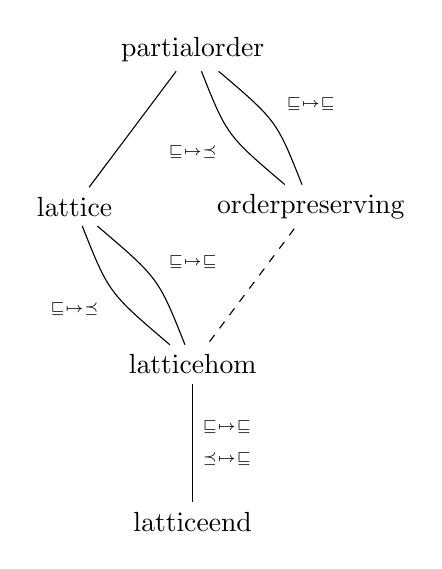
\begin{tikzpicture}
  \node (o) at (0,0) {\isa{partial{\isacharunderscore}order}};
  \node (oh) at (1.5,-2) {\isa{order{\isacharunderscore}preserving}};
  \node (oh1) at (1.5,-0.7) {$\scriptscriptstyle \sqsubseteq \mapsto \sqsubseteq$};
  \node (oh2) at (0,-1.3) {$\scriptscriptstyle \sqsubseteq \mapsto \preceq$};
  \node (l) at (-1.5,-2) {\isa{lattice}};
  \node (lh) at (0,-4) {\isa{lattice{\isacharunderscore}hom}};
  \node (lh1) at (0,-2.7) {$\scriptscriptstyle \sqsubseteq \mapsto \sqsubseteq$};
  \node (lh2) at (-1.5,-3.3) {$\scriptscriptstyle \sqsubseteq \mapsto \preceq$};
  \node (le) at (0,-6) {\isa{lattice{\isacharunderscore}end}};
  \node (le1) at (0,-4.8)
    [anchor=west]{$\scriptscriptstyle \sqsubseteq \mapsto \sqsubseteq$};
  \node (le2) at (0,-5.2)
    [anchor=west]{$\scriptscriptstyle \preceq \mapsto \sqsubseteq$};
  \draw (o) -- (l);
  \draw[dashed] (oh) -- (lh);
  \draw (lh) -- (le);
  \draw (o) .. controls (oh1.south west) .. (oh);
  \draw (o) .. controls (oh2.north east) .. (oh);
  \draw (l) .. controls (lh1.south west) .. (lh);
  \draw (l) .. controls (lh2.north east) .. (lh);
\end{tikzpicture}
\end{center}
\hrule
\caption{Hierarchy of Homomorphism Locales.}
\label{fig:hom}
\end{figure}%
\end{isamarkuptext}%
\isamarkuptrue%
%
\begin{isamarkuptext}%
It can be shown easily that a lattice homomorphism is order
  preserving.  As the final example of this section, a locale
  interpretation is used to assert this:%
\end{isamarkuptext}%
\isamarkuptrue%
\ \ \isacommand{sublocale}\isamarkupfalse%
\ lattice{\isacharunderscore}hom\ {\isasymsubseteq}\ order{\isacharunderscore}preserving%
\isadelimproof
\ %
\endisadelimproof
%
\isatagproof
\isacommand{proof}\isamarkupfalse%
\ unfold{\isacharunderscore}locales\isanewline
\ \ \ \ \isacommand{fix}\isamarkupfalse%
\ x\ y\isanewline
\ \ \ \ \isacommand{assume}\isamarkupfalse%
\ {\isachardoublequoteopen}x\ {\isasymsqsubseteq}\ y{\isachardoublequoteclose}\isanewline
\ \ \ \ \isacommand{then}\isamarkupfalse%
\ \isacommand{have}\isamarkupfalse%
\ {\isachardoublequoteopen}y\ {\isacharequal}\ {\isacharparenleft}x\ {\isasymsqunion}\ y{\isacharparenright}{\isachardoublequoteclose}\ \isacommand{by}\isamarkupfalse%
\ {\isacharparenleft}simp\ add{\isacharcolon}\ le{\isachardot}join{\isacharunderscore}connection{\isacharparenright}\isanewline
\ \ \ \ \isacommand{then}\isamarkupfalse%
\ \isacommand{have}\isamarkupfalse%
\ {\isachardoublequoteopen}{\isasymphi}\ y\ {\isacharequal}\ {\isacharparenleft}{\isasymphi}\ x\ {\isasymsqunion}{\isacharprime}\ {\isasymphi}\ y{\isacharparenright}{\isachardoublequoteclose}\ \isacommand{by}\isamarkupfalse%
\ {\isacharparenleft}simp\ add{\isacharcolon}\ hom{\isacharunderscore}join\ {\isacharbrackleft}symmetric{\isacharbrackright}{\isacharparenright}\isanewline
\ \ \ \ \isacommand{then}\isamarkupfalse%
\ \isacommand{show}\isamarkupfalse%
\ {\isachardoublequoteopen}{\isasymphi}\ x\ {\isasympreceq}\ {\isasymphi}\ y{\isachardoublequoteclose}\ \isacommand{by}\isamarkupfalse%
\ {\isacharparenleft}simp\ add{\isacharcolon}\ le{\isacharprime}{\isachardot}join{\isacharunderscore}connection{\isacharparenright}\isanewline
\ \ \isacommand{qed}\isamarkupfalse%
%
\endisatagproof
{\isafoldproof}%
%
\isadelimproof
%
\endisadelimproof
%
\begin{isamarkuptext}%
Theorems and other declarations --- syntax, in particular --- from
  the locale \isa{order{\isacharunderscore}preserving} are now active in \isa{lattice{\isacharunderscore}hom}, for example
  \isa{hom{\isacharunderscore}le}:
  \begin{isabelle}%
\ \ {\isacharquery}x\ {\isasymsqsubseteq}\ {\isacharquery}y\ {\isasymLongrightarrow}\ {\isasymphi}\ {\isacharquery}x\ {\isasympreceq}\ {\isasymphi}\ {\isacharquery}y%
\end{isabelle}%
\end{isamarkuptext}%
\isamarkuptrue%
%
\isamarkupsection{Further Reading%
}
\isamarkuptrue%
%
\begin{isamarkuptext}%
More information on locales and their interpretation is
  available.  For the locale hierarchy of import and interpretation
  dependencies see \cite{Ballarin2006a}; interpretations in theories
  and proofs are covered in \cite{Ballarin2006b}.  In the latter, I
  show how interpretation in proofs enables to reason about families
  of algebraic structures, which cannot be expressed with locales
  directly.

  Haftmann and Wenzel \cite{HaftmannWenzel2007} overcome a restriction
  of axiomatic type classes through a combination with locale
  interpretation.  The result is a Haskell-style class system with a
  facility to generate ML and Haskell code.  Classes are sufficient for
  simple specifications with a single type parameter.  The locales for
  orders and lattices presented in this tutorial fall into this
  category.  Order preserving maps, homomorphisms and vector spaces,
  on the other hand, do not.

  The locales reimplementation for Isabelle 2009 provides, among other
  improvements, a clean intergration with Isabelle/Isar's local theory
  mechnisms, which are described in \cite{HaftmannWenzel2009}.

  The original work of Kamm\"uller on locales \cite{KammullerEtAl1999}
  may be of interest from a historical perspective.  The mathematical
  background on orders and lattices is taken from Jacobson's textbook
  on algebra \cite[Chapter~8]{Jacobson1985}.

  The sources of this tutorial, which include all proofs, are
  available with the Isabelle distribution at
  \url{http://isabelle.in.tum.de}.%
\end{isamarkuptext}%
\isamarkuptrue%
%
\begin{isamarkuptext}%
\begin{table}
\hrule
\vspace{2ex}
\begin{center}
\begin{tabular}{l>$c<$l}
  \multicolumn{3}{l}{Miscellaneous} \\

  \textit{attr-name} & ::=
  & \textit{name} $|$ \textit{attribute} $|$
    \textit{name} \textit{attribute} \\
  \textit{qualifier} & ::=
  & \textit{name} [``\textbf{?}'' $|$ ``\textbf{!}''] \\[2ex]

  \multicolumn{3}{l}{Context Elements} \\

  \textit{fixes} & ::=
  & \textit{name} [ ``\textbf{::}'' \textit{type} ]
    [ ``\textbf{(}'' \textbf{structure} ``\textbf{)}'' $|$
    \textit{mixfix} ] \\
\begin{comment}
  \textit{constrains} & ::=
  & \textit{name} ``\textbf{::}'' \textit{type} \\
\end{comment}
  \textit{assumes} & ::=
  & [ \textit{attr-name} ``\textbf{:}'' ] \textit{proposition} \\
\begin{comment}
  \textit{defines} & ::=
  & [ \textit{attr-name} ``\textbf{:}'' ] \textit{proposition} \\
  \textit{notes} & ::=
  & [ \textit{attr-name} ``\textbf{=}'' ]
    ( \textit{qualified-name} [ \textit{attribute} ] )$^+$ \\
\end{comment}

  \textit{element} & ::=
  & \textbf{fixes} \textit{fixes} ( \textbf{and} \textit{fixes} )$^*$ \\
\begin{comment}
  & |
  & \textbf{constrains} \textit{constrains}
    ( \textbf{and} \textit{constrains} )$^*$ \\
\end{comment}
  & |
  & \textbf{assumes} \textit{assumes} ( \textbf{and} \textit{assumes} )$^*$ \\[2ex]
%\begin{comment}
%  & |
%  & \textbf{defines} \textit{defines} ( \textbf{and} \textit{defines} )$^*$ \\
%  & |
%  & \textbf{notes} \textit{notes} ( \textbf{and} \textit{notes} )$^*$ \\
%\end{comment}

  \multicolumn{3}{l}{Locale Expressions} \\

  \textit{pos-insts} & ::=
  & ( \textit{term} $|$ ``\textbf{\_}'' )$^*$ \\
  \textit{named-insts} & ::=
  & \textbf{where} \textit{name} ``\textbf{=}'' \textit{term}
  ( \textbf{and} \textit{name} ``\textbf{=}'' \textit{term} )$^*$ \\
  \textit{instance} & ::=
  & [ \textit{qualifier} ``\textbf{:}'' ]
    \textit{qualified-name} ( \textit{pos-insts} $|$ \textit{named-inst} ) \\
  \textit{expression}  & ::= 
  & \textit{instance} ( ``\textbf{+}'' \textit{instance} )$^*$
    [ \textbf{for} \textit{fixes} ( \textbf{and} \textit{fixes} )$^*$ ] \\[2ex]

  \multicolumn{3}{l}{Declaration of Locales} \\

  \textit{locale} & ::=
  & \textit{element}$^+$ \\
  & | & \textit{expression} [ ``\textbf{+}'' \textit{element}$^+$ ] \\
  \textit{toplevel} & ::=
  & \textbf{locale} \textit{name} [ ``\textbf{=}''
    \textit{locale} ] \\[2ex]

  \multicolumn{3}{l}{Interpretation} \\

  \textit{equation} & ::= & [ \textit{attr-name} ``\textbf{:}'' ]
    \textit{prop} \\
  \textit{equations} & ::= &  \textbf{where} \textit{equation} ( \textbf{and}
    \textit{equation} )$^*$  \\
  \textit{toplevel} & ::=
  & \textbf{sublocale} \textit{name} ( ``$<$'' $|$
    ``$\subseteq$'' ) \textit{expression} \textit{proof} \\
  & |
  & \textbf{interpretation}
    \textit{expression} [ \textit{equations} ] \textit{proof} \\
  & |
  & \textbf{interpret}
    \textit{expression} \textit{proof} \\[2ex]

  \multicolumn{3}{l}{Diagnostics} \\

  \textit{toplevel} & ::=
  & \textbf{print\_locales} \\
  & | & \textbf{print\_locale} [ ``\textbf{!}'' ] \textit{locale} \\
  & | & \textbf{print\_interps} \textit{locale}
\end{tabular}
\end{center}
\hrule
\caption{Syntax of Locale Commands.}
\label{tab:commands}
\end{table}%
\end{isamarkuptext}%
\isamarkuptrue%
%
\begin{isamarkuptext}%
\textbf{Revision History.}  For the present third revision,
  which was completed in October 2009, much of the explanatory text
  has been rewritten.  In addition, inheritance of interpretation
  equations, which was not available for Isabelle 2009, but in the
  meantime has been implemented, is illustrated.  The second revision
  accommodates changes introduced by the locales reimplementation for
  Isabelle 2009.  Most notably, in complex specifications
  (\emph{locale expressions}) renaming has been generalised to
  instantiation.%
\end{isamarkuptext}%
\isamarkuptrue%
%
\begin{isamarkuptext}%
\textbf{Acknowledgements.}  Alexander Krauss, Tobias Nipkow,
  Randy Pollack, Christian Sternagel and Makarius Wenzel have made
  useful comments on earlier versions of this document.%
\end{isamarkuptext}%
\isamarkuptrue%
%
\isadelimtheory
%
\endisadelimtheory
%
\isatagtheory
\isacommand{end}\isamarkupfalse%
%
\endisatagtheory
{\isafoldtheory}%
%
\isadelimtheory
%
\endisadelimtheory
\isanewline
\end{isabellebody}%
%%% Local Variables:
%%% mode: latex
%%% TeX-master: "root"
%%% End:
